\capitulo{5}{Aspectos relevantes del desarrollo del proyecto}

%Este apartado pretende recoger los aspectos más interesantes del desarrollo del proyecto, comentados por los autores del mismo.
%Debe incluir desde la exposición del ciclo de vida utilizado, hasta los detalles de mayor relevancia de las fases de análisis, diseño e implementación.
%Se busca que no sea una mera operación de copiar y pegar diagramas y extractos del código fuente, sino que realmente se justifiquen los caminos de solución que se han tomado, especialmente aquellos que no sean triviales.
%Puede ser el lugar más adecuado para documentar los aspectos más interesantes del diseño y de la implementación, con un mayor hincapié en aspectos tales como el tipo de arquitectura elegido, los índices de las tablas de la base de datos, normalización y desnormalización, distribución en ficheros3, reglas de negocio dentro de las bases de datos (EDVHV GH GDWRV DFWLYDV), aspectos de desarrollo relacionados con el WWW...
%Este apartado, debe convertirse en el resumen de la experiencia práctica del proyecto, y por sí mismo justifica que la memoria se convierta en un documento útil, fuente de referencia para los autores, los tutores y futuros alumnos.

En este apartado se va a recoger el ciclo de vida del proyecto, detallando los aspectos más relevantes que se han tratado y como se han resuelto las diferentes  dificultades encontradas a lo largo de su desarrollo.

Se irán presentando diferentes secciones que concuerdan con el orden cronológico seguido en el proyecto y muestran la justificación de las decisiones tomadas.

\section{Propuesta del proyecto}

La propuesta de este proyecto consistía en crear una aplicación Android para el reconocimiento de setas que se dividía en las siguientes 3 tareas principales:

\begin{itemize}
	\item{Clasificador de imágenes:} La tarea principal pedida para realizar este proyecto era la de construir un clasificador visual de imágenes que a través de la foto realizada a una seta nos devolviera un listado de las especies más probables.
	\item{Web Semántica:} Conseguir información a través de una web semántica para documentar las especies de setas incluidas en el clasificador.
	\item{Clave dicotómica:} Incorporar una clave dicotómica que reforzara la tarea del clasificador para el reconocimiento de la especie.
\end{itemize}

Ante estas tareas se empezó a investigar que alternativas había para construir una aplicación que fuera lo suficientemente precisa y de fácil uso para el usuario. Se barajaron las siguientes posibilidades:

\begin{itemize}
	\item{Incorporar sólo un clasificador visual:} Si sólo se implementaba un clasificador visual en la aplicación, esta sería muy fácil de usar pero sería poco precisa ya que clasificar la especie de una seta por una única foto es una tarea casi imposible. 
	\item{Clasificador visual con elección manual entre las candidatas:} La idea de esta propuesta es la de mostrar al usuario un listado con las cinco especies más probables clasificadas para esa foto y que este las pueda comparar mediante fotografías proporcionadas por la aplicación de esas especies con su foto. Esta propuesta puede ser un poco más fiable pero depende de los conocimientos del usuario y la hace más compleja.
	\item{Clave dicotómica única:} Incluir una clave dicotómica aislada del clasificador podía proporcionar una gran fiabilidad pero suelen ser claves de difícil uso para el usuario.
	\item{Clave dicotómica más el clasificador:} Esta propuesta consistía en filtrar las preguntas de la clave dicotómica en base a los resultados obtenidos por el clasificador de imágenes.
\end{itemize}

Con estas propuestas en mente se empezó a estudiar como se podía implementar el clasificador de imágenes y como podíamos implementar las diferentes propuestas en base a lo que se iba desarrollando.

\section{¿Cómo implementar el clasificador?}

Se decidió empezar por la tarea de generar el clasificador de imágenes ya que era la tarea más complicada de realizar y de la que dependían las demás tareas. En la asignatura de minería de datos ya había adquirido conocimientos sobre como entrenar y usar clasificadores de imágenes pero ahora surgía la duda de como hacer esto mismo pero en una plataforma nueva para mí que era Android. En las primeras reuniones del proyecto los profesores me propusieron las siguientes posibilidades para realizarlo:

\begin{itemize}
	\item Entrenar un clasificador de imágenes desde cero que se ejecutara en un servidor Web y mostrara los resultados en el teléfono móvil.
	\item Seguir la propuesta anterior pero reentrenando una red neuronal en vez de entrenar un modelo desde cero.
	\item Reentrenar los nuevos modelos Mobilenet mediante Tensorflow, lo que nos permitiría ejecutar los clasificadores en el propio dispositivo móvil.
\end{itemize}

Elegí empezar por estudiar la tercera propuesta y ver si era posible ejecutar los modelos en el propio teléfono móvil. Esta propuesta tiene la ventaja de que el usuario no necesita estar conectado a un servidor Web, característica importante si pensamos que esta aplicación se usara en zonas con poca cobertura.

La preocupación principal era saber si los modelos se iban a poder ejecutar en el propio móvil de una manera rápida, ya que es un proceso costoso, y que nos proporcionara los resultados deseados. Después de estudiar la tecnología Tensorflow y cómo implementarla en una aplicación Android probé varios varios modelos preentrenados de prueba que proporcionan en los ejemplos de Tensorflow\footnote{\url{https://github.com/tensorflow/tensorflow/tree/master/tensorflow/examples/android}} y vi que la aplicación se ejecutaba correctamente en diferentes modelos de móvil simulados y en mi propio teléfono.

Esta etapa del proyecto me permitió empezar a familiarizarme con el entorno de programación Android Studio y con las librerías de Tensorflow.

Después de realizar pruebas con modelos preentrenados y ejemplos empecé a estudiar como poder entrenar mi propio modelo de Mobilenet o Inception, con nuestro repositorio de imágenes de setas, para que diferenciara entre las diferentes especies. La solución la encontré en el mismo repositorio de Github\footnote{\url{https://github.com/tensorflow/tensorflow/tree/master/tensorflow/examples/image_retraining}} de Tensoflow en el que proporcionan un script en python (\textit{retrain.py}) para reentrenar ambos modelos pudiendo modificar gran variedad de parámetros y ajustes para crear un modelo personalizado.

Gracias a estos scripts y a los ejemplos encontrados de Tensorflow en Android conseguí reentrenar los primeros modelos y clasificar las primeras imágenes en el propio móvil.

Las imágenes usadas para entrenar los modelos se sacaron de los repositorios Imagenet\footnote{\url{http://www.image-net.org/index}} y Enciclopedia of Life\footnote{\url{http://eol.org}}, recopilando aproximadamente entre 30 y 80 fotos por cada especie de seta. En total se han usado 9400 fotografías para reentrenar el clasificador completo divididas en 171 especies de setas.

Las primeras pruebas se ejecutaron con un modelo Mobilenet v1-224 reentrenado, que diferenciaba 118 especies de setas, en un teléfono móvil Samsung galaxy S5. La aplicación lograba ejecutarse fluidamente y se consiguió una precisión (61,5\%) \ref{figMobilenet1} en la validación cruzada con 4000 pasos de reentrenamiento:

\begin{figure}[h]
    \begin{center}%
        \begin{center}%
          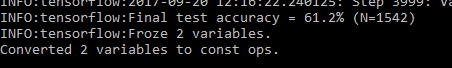
\includegraphics[width=1\textwidth]{mobilenet1}%
          \caption{Mobilenet v1-224, 4000 \textit{steps}, 118 especies.}%
          \label{figMobilenet1}%
        \end{center}%
  	\end{center}%
\end{figure}%

Aunque la precisión de estos modelos no sea relativamente alta, nos basta con que la especie correcta se encuentre entre los cinco primeros resultados del clasificador, ya que este clasificador se complementará con la clave dicotómica.

\section{¿Qué modelo de clasificador usar?}

Para elegir el modelo a usar se tuvieron que tener en cuenta diferentes factores como el peso del modelo, su carga de computo y su precisión. En teoría el modelo Inception es más preciso que el Mobilenet pero requiere mayor capacidad de computo y espacio de almacenamiento, recursos que son limitados en los teléfonos móviles.

Para Mobilenet contábamos con los modelos mostrados en la figura \ref{figComparativaMobilenet} mientras que de Inception solo podía reentrenar el modelo Inception v3.

\begin{figure}[h]
    \begin{center}%
        \begin{center}%
          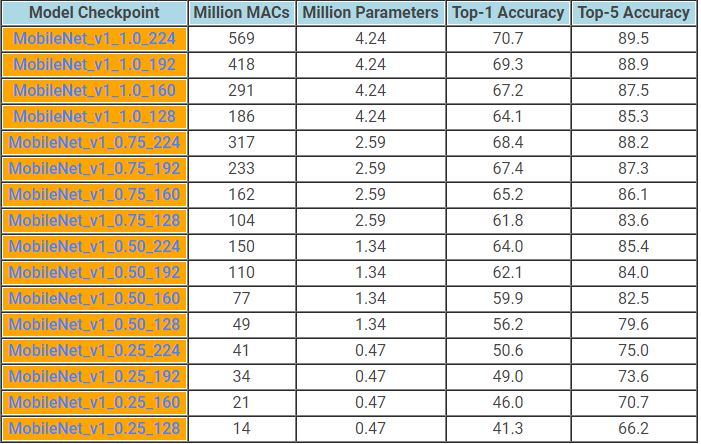
\includegraphics[width=1\textwidth]{comparativaMobilenet}%
          \caption{Comparativa modelos Mobilenet}%
          \label{figComparativaMobilenet}%
        \end{center}%
  	\end{center}%
\end{figure}%
\newpage
Se realizaron pruebas con los diferentes modelos y al final opté por usar el modelo Mobilenet v1 224 ya que se ejecutaba de forma suficientemente fluida y proporciona una precision superior a los demás modelos Mobilenet. 

Respecto al modelo Inception su peso era de 75 Megabytes en contra de los 17 Megabytes que ocupaba el modelo Mobilenet y los resultados obtenidos \ref{figInception1} en validación cruzada eran parecidos entrenados en las mismas condiciones. 

%https://opensource.googleblog.com/2017/06/mobilenets-open-source-models-for.html
\begin{figure}[h]
    \begin{center}%
        \begin{center}%
          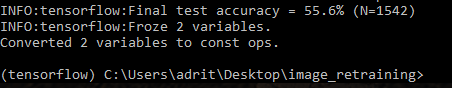
\includegraphics[width=1\textwidth]{inception1}%
          \caption{Inception v3, 4000 \textit{steps}, 118 especies.}%
          \label{figInception1}%
        \end{center}%
  	\end{center}%
\end{figure}%

Una vez elegido el modelo se procedió a escalar el modelo aumentando el número de especies a diferenciar, pasando de clasificar 118 especies a un total de 171. Este aumento provoco un ligero descenso en la precisión del clasificador que se solvento aplicando técnicas de Data augmentation a la hora de entrenar el modelo. La precisión obtenida final fue de un 59,4\% \ref{figMobilenet2} en validación cruzada de media entre todas las categorías de especies de setas.

Se probó a aumentar el número de pasos de entrenamiento pero esto no provocaba un ascenso de la precisión sino que se mantenía constante y provocaba el riesgo de que se sobre-entrenara el modelo por lo que se decidió dejar el parámetro en 4000 pasos.

El tiempo necesario para entrenar este modelos con un procesador i7 4790, fue de 5 horas 55 minutos.

\begin{figure}[h]
    \begin{center}%
        \begin{center}%
          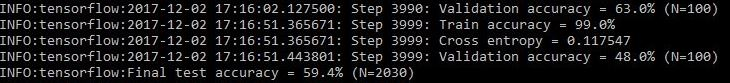
\includegraphics[width=1\textwidth]{mobilenet2}%
          \caption[Mobilenet v1-224, 4000 \textit{steps}, 171 especies]{Mobilenet v1-224, 4000 \textit{steps}, 171 especies, con data augmentation.}%
          \label{figMobilenet2}%
        \end{center}%
  	\end{center}%
\end{figure}%

\section{Web Semántica}

La siguiente tarea que se decidió afrontar después de implementar el clasificador de imágenes fue la parte de Web semántica. En esta tarea había que recopilar información de las diferentes especies de setas, de alguna Web semántica, con el objetivo de crear fichas para cada especie que pudiera consultar el usuario en cualquier momento.

La principal dificultad que se encontró en este apartado y que determinó el uso de la DBpedia como Web semántica, fue encontrar un repositorio que contuviera información suficiente de todas las especies sin excepción.El alto número de especies que podía clasificar la aplicación dificultaba esta tarea. Este requisito era necesario para automatizar la extracción de datos y que todas las especies tuvieran su ficha de información.

La DBpedia era la única que recopilaba información suficiente de todas las especies al completo y nos proporcionaba la información mínima deseada como era una descripción de la especie y la comestibilidad de esta.

Otra opción que se contempló fue la de usar \textit{web scraping} en vez de consultas a una web semántica, pero esta opción se descarto ya que no se logró encontrar un repositorio con todas la especies y que contuviera más información que la que proporcionaba por la DBpedia.

Gracias al lenguaje de consultas SparQL y la librería Apache Jena para Java se implemento un programa en Windows que realizaba consultas a la DBpedia y nos devolvía la información necesaria.

El siguiente problema a afrontar era como almacenar y transferir esta información a la aplicación Android. Después de estudiar diferentes bases de datos se opto por usar la base de datos SQLite. Esta base de datos tiene soporte tanto para Android como para Windows por lo que es fácil exportar los datos de una plataforma a otra. Además no requiere de configuración de usuarios ni conexiones lo que simplifica su uso. Aunque proporcione una funcionalidad básica, esta base de datos nos permitía almacenar nuestra información y cumplía con los requisitos de la aplicación.

Para mostrar imágenes comparativas de las especies se usaron una parte de las imágenes ya recopiladas, que se habían usado para entrenar el clasificador. Estas imágenes se formatearon en una resolución menor que la original para ahorrar espacio en la aplicación. Estas imágenes se almacenaron dentro de la propia estructura de la aplicación Android.

Una vez recopilada la información de las diferentes especies, la aplicación era capaz de clasificar las cinco especies más probables respecto a la imagen de la seta introducida, mostrar imágenes comparativas de las especies y mostrar información de cada especie.

De cara a la internacionalización de la aplicación se implementó un método que tradujera automáticamente mediante el traductor de Google la información de la DBpedia en caso de no estar disponible en el idioma deseado. Por ejemplo, había veces que la información no se encontraba disponible en Español por lo que se traducía desde la versión en inglés.

\section{Clave dicotómica}

El último apartado a tratar era el de implementar una clave dicotómica que nos permitiera diferenciar entre todos los géneros contenidos en el clasificador. Esta tarea tenia las dos siguientes dificultades:

\begin{itemize}
	\item Conseguir una clave dicotómica que discriminara entre todos los géneros de especies del clasificador.
	\item Estructurar esa clave dicotómica de una forma que se pudiera manejar para implementarse en la aplicación Android.
\end{itemize}

Después de buscar en diferentes páginas web, se encontró una (\url{http://www.avelinosetas.info/claves.php}) que contenía una serie de claves dicotómicas para diferentes especies y una clave que discriminaba entre 108 géneros de setas. De las claves encontradas fue la que más géneros contemplaba. Para que los géneros de la clave y del clasificador coincidieran se recopilaron imágenes de las especies que no se contemplaban en el clasificador para reentrenarlo y que pudiera discriminar entre 171 especies distintas.

Esta solución tiene la limitación de que el número de setas discriminado por el clasificador no es el mismo que el de la clave dicotómica.

Para extraer las claves de la página Web se desarrollo un programa en Java que mediante técnicas de Web Scraping extrajera las claves dicotómicas y las almacenar en estructuras de datos que nos permitieran usarlas para nuestra aplicación Android.

Además de la clave general de géneros, se extrajeron las claves dicotómicas disponibles para diferenciar entre especies concretas dentro de un mismo género. Actualmente la aplicación dispone de 39 claves dicotómicas de géneros concretos para clasificar la especie concreta.

Esta tarea se pudo automatizar mediante la herramienta Jaunt para Java revisando el código html de la página Web.

\section{Aspectos de diseño}

Para diseñar la interfaz de la aplicación se siguieron las recomendaciones de Material Design\footnote{\url{https://material.io/guidelines/}}. Se elaboró un prototipado inicial de las diferentes actividades y a partir de ahí se fue elaborando la interfaz final integrando los diferentes modulos de la aplicación (clasificador de imágenes, muestra de información y las claves dicotómicas).

Se han intentado usar colores planos siguiendo las indicaciones de Material Design así como iconos intuitivos para los diferentes botones de la aplicación.

La aplicación está desarrollada para que se pueda visualizar en vertical como en horizontal. Además se han usado medidas relativas de los elementos para que la aplicación se pueda adaptar a diferentes tamaños de pantalla.

La aplicación cuenta con un menú lateral que nos permite navegar desde cualquier punto de la aplicación a las opciones principales.

Se ha traducido la aplicación al Inglés y Español traduciendo tanto textos extraídos de la DBpedia cómo las cuarenta claves dicotómicas implementadas. El idioma de la aplicación se puede cambiar en cualquier momento desde la opción del menú lateral.

Cada actividad de la aplicación cuenta con un menú de ayuda que explica la funcionalidad completa de la actividad en la que te encuentras. El menú lateral cuenta con su propia ayuda.

Respecto al tamaño de la aplicación, este se ha conseguido reducir a un total de 42,6 Megabytes. Para ello se tuvieron que formatear las imágenes de las 171 especies de setas (5 imágenes por especie) a una resolución menor, así como usar el modelo Mobilenet en vez del Inception.









